\documentclass[11pt]{article}

\usepackage[a4paper,margin=0.75in]{geometry}
\usepackage{amsmath,amssymb}
\usepackage{graphicx}
\usepackage{booktabs}
\usepackage{array}
\usepackage{float}
\usepackage{hyperref}
\usepackage{enumitem}
\usepackage{xcolor}
\usepackage{tikz}
\usetikzlibrary{positioning,arrows.meta,shapes.geometric}

\setlist{nosep}
\renewcommand{\arraystretch}{1.3}

\tikzset{
layer/.style={
draw,
rounded corners,
minimum width=2.2cm,
minimum height=0.9cm,
align=center,
fill=blue!10
},
arrow/.style={
-{Latex[length=3mm]},
thick
}
}

\begin{document}

%%%%%%%%%%%%%%%%%%%%%%%%%%%%%%%%%%%%%%%%%%%%%%%%%%%%%%%%%%%%

\begin{center}

{\Large\textbf{Shiv Nadar University Chennai}}

\vspace{3mm}

{\large\textbf{CS3807 -- Deep Learning Laboratory}}

\vspace{3mm}

{\Large\textbf{Experiment 4}}

\vspace{2mm}

{\Large\textbf{Comparative Study of Deep Convolutional Neural}}

{\Large\textbf{Network Architectures Using Transfer Learning}}

\end{center}

\vspace{5mm}

\begin{tabular}{|p{4cm}|p{8cm}|p{2cm}|}
\hline
Degree \& Branch &
B.Tech Artificial Intelligence \& Data Science &
Semester V\\
\hline
Subject Code \& Name &
CS3807 -- Deep Learning Laboratory &
AY: 2026--27\\
\hline
\end{tabular}

%%%%%%%%%%%%%%%%%%%%%%%%%%%%%%%%%%%%%%%%%%%%%%%%%%%%%%%%%%%%

\section*{1. Objective}

The objectives of this experiment are

\begin{itemize}

\item Study the evolution of deep CNN architectures.

\item Compare LeNet-5, AlexNet, VGG16, GoogleNet and ResNet.

\item Understand transfer learning.

\item Fine tune pretrained CNN models.

\item Compare classification performance of different architectures.

\end{itemize}

%%%%%%%%%%%%%%%%%%%%%%%%%%%%%%%%%%%%%%%%%%%%%%%%%%%%%%%%%%%%

\section*{2. Learning Outcomes}

After completing this experiment students will be able to

\begin{enumerate}

\item Explain modern CNN architectures.

\item Differentiate LeNet, AlexNet, VGG16, GoogleNet and ResNet.

\item Implement transfer learning.

\item Fine tune pretrained CNN models.

\item Compare CNN architectures using performance metrics.

\end{enumerate}

%%%%%%%%%%%%%%%%%%%%%%%%%%%%%%%%%%%%%%%%%%%%%%%%%%%%%%%%%%%%

\section*{3. Introduction}

Deep Convolutional Neural Networks have become the dominant models for
computer vision applications because they automatically learn hierarchical
features directly from raw image data, removing the need for hand-engineered
descriptors. The evolution of CNN architectures over the past two decades has
been driven by three competing goals: improving classification accuracy,
reducing computational and memory cost, and making very deep networks
trainable in practice.

The progression of CNN architectures began with LeNet-5 and has evolved
through AlexNet, VGGNet, GoogleNet, and ResNet, with transfer learning later
emerging as a practical way to reuse the representations learned by these
large networks on new, smaller datasets. This experiment studies that
progression directly: five architectures are evaluated on the CIFAR-10
dataset, and one of them (MobileNetV2) is taken through a complete
transfer-learning and fine-tuning pipeline.

%%%%%%%%%%%%%%%%%%%%%%%%%%%%%%%%%%%%%%%%%%%%%%%%%%%%%%%%%%%%

\section*{4. Evolution of CNN Architectures}

\begin{center}

\begin{tabular}{|l|l|p{7cm}|}

\hline

Model & Year & Major Contribution\\

\hline

LeNet-5 & 1998 & First practical convolutional neural network\\

\hline

AlexNet & 2012 & ReLU activation, Dropout and GPU training\\

\hline

VGG16 & 2014 & Uniform $3\times3$ convolution filters\\

\hline

GoogleNet & 2014 & Inception modules for multi-scale feature extraction\\

\hline

ResNet & 2015 & Residual learning using skip connections\\

\hline

\end{tabular}

\end{center}

%%%%%%%%%%%%%%%%%%%%%%%%%%%%%%%%%%%%%%%%%%%%%%%%%%%%%%%%%%%%

\section*{5. LeNet-5}

LeNet-5 was proposed by Yann LeCun in 1998 for handwritten digit recognition.
It consists of two convolution layers, two average pooling layers and fully
connected layers. It demonstrated that convolutional networks could
automatically learn discriminative image features without relying on
handcrafted feature extraction -- a departure from the classical computer
vision pipelines of its time.

Advantages

\begin{itemize}
\item Small number of parameters
\item Fast training
\item Suitable for OCR
\end{itemize}

%%%%%%%%%%%%%%%%%%%%%%%%%%%%%%%%%%%%%%%%%%%%%%%%%%%%%%%%%%%%

\section*{6. AlexNet}

AlexNet won the ImageNet Large Scale Visual Recognition Challenge in 2012 by
a wide margin, reducing the top-5 classification error substantially compared
to prior approaches. Its success is generally credited to a combination of
architectural and training choices rather than any single innovation.

Major innovations

\begin{itemize}
\item ReLU activation
\item Dropout
\item GPU implementation
\item Data augmentation
\end{itemize}

%%%%%%%%%%%%%%%%%%%%%%%%%%%%%%%%%%%%%%%%%%%%%%%%%%%%%%%%%%%%

\section*{7. VGG16}

VGG16 showed that stacking multiple small $3\times3$ convolution filters
could match or outperform the larger filters used in earlier architectures,
while also increasing the effective depth of the network.

Advantages

\begin{itemize}
\item Excellent feature extraction
\item Simple, uniform architecture
\item High classification accuracy
\end{itemize}

%%%%%%%%%%%%%%%%%%%%%%%%%%%%%%%%%%%%%%%%%%%%%%%%%%%%%%%%%%%%

\section*{8. Comparison of Architectures}

\begin{center}

\begin{tabular}{|l|c|c|p{5.5cm}|}

\hline

Architecture & Depth & Parameters & Main Contribution\\

\hline

LeNet-5 & 7 & 60K & First CNN\\

\hline

AlexNet & 8 & 61M & ReLU + Dropout\\

\hline

VGG16 & 16 & 138M & Deep $3\times3$ filters\\

\hline

GoogleNet & 22 & 6.8M & Inception Modules\\

\hline

ResNet50 & 50 & 25.6M & Residual Learning\\

\hline

\end{tabular}

\end{center}

%%%%%%%%%%%%%%%%%%%%%%%%%%%%%%%%%%%%%%%%%%%%%%%%%%%%%%%%%%%%

\section*{9. GoogleNet (Inception Network)}

GoogleNet, proposed by Szegedy et al. in 2014, introduced the Inception
Module, which performs multiple convolution operations in parallel using
different filter sizes. Rather than committing to a single kernel size at
each layer, GoogleNet simultaneously applies $1\times1$, $3\times3$,
$5\times5$ convolutions and max pooling, then concatenates the results to
obtain a multi-scale feature representation.

The use of $1\times1$ convolutions before the larger kernels reduces the
number of trainable parameters and the overall computational cost of the
module.

Advantages

\begin{itemize}
\item Multi-scale feature extraction.
\item Fewer parameters than VGG16.
\item High computational efficiency.
\item Strong classification performance.
\end{itemize}

%%%%%%%%%%%%%%%%%%%%%%%%%%%%%%%%%%%%%%%%%%%%%%%%%%%%%%%%%%%%

\section*{10. ResNet}

Increasing CNN depth often causes the \textbf{vanishing gradient problem},
making optimization difficult. ResNet solves this issue using
\textbf{skip (residual) connections}, allowing gradients to flow directly
through the network.

Instead of learning

\[
H(x)
\]

ResNet learns

\[
F(x)=H(x)-x
\]

thus,

\[
Output = F(x)+x
\]

where

\begin{itemize}
\item $F(x)$ = Residual Mapping
\item $x$ = Identity Mapping
\end{itemize}

\begin{figure}[H]
\centering

\resizebox{0.75\textwidth}{!}{%
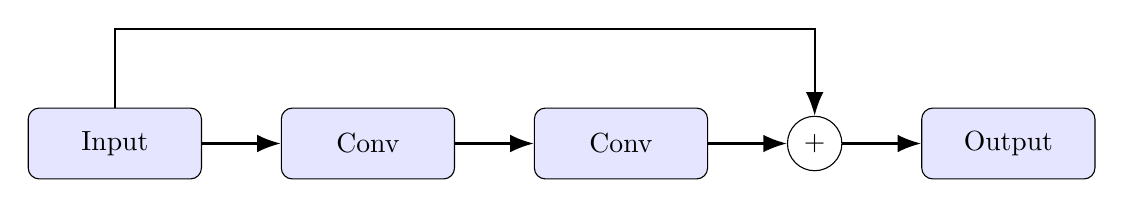
\begin{tikzpicture}[node distance=1cm]

\node[layer](input){Input};

\node[layer,right=of input](conv1){Conv};

\node[layer,right=of conv1](conv2){Conv};

\node[circle,draw,right=of conv2](add){+};

\node[layer,right=of add](output){Output};

\draw[arrow](input)--(conv1);
\draw[arrow](conv1)--(conv2);
\draw[arrow](conv2)--(add);
\draw[arrow](add)--(output);

\draw[arrow]
(input)
|-([yshift=10mm]conv2.north)
-| (add.north);

\end{tikzpicture}%
}

\caption{Residual Block in ResNet}
\end{figure}

Advantages

\begin{itemize}
\item Eliminates vanishing gradients.
\item Enables very deep neural networks.
\item Faster convergence.
\item High ImageNet accuracy.
\end{itemize}

%%%%%%%%%%%%%%%%%%%%%%%%%%%%%%%%%%%%%%%%%%%%%%%%%%%%%%%%%%%%

\section*{11. Dilated Convolution}

Dilated convolution (also called atrous convolution) increases the
receptive field of a filter without increasing its parameter count, by
introducing gaps between kernel elements.

For a standard convolution,

\[
D=1
\]

For dilated convolution,

\[
D>1
\]

Example

\[
\begin{bmatrix}
1 & 0 & 2\\
0 & 3 & 0\\
4 & 0 & 5
\end{bmatrix}
\]

where the inserted zeros indicate the gaps introduced by the dilation.

Applications

\begin{itemize}
\item Semantic segmentation
\item Medical image analysis
\item Satellite imagery
\item Object localization
\end{itemize}

%%%%%%%%%%%%%%%%%%%%%%%%%%%%%%%%%%%%%%%%%%%%%%%%%%%%%%%%%%%%

\section*{12. Transpose Convolution}

Transpose convolution increases the spatial dimensions of a feature map.
Unlike pooling, which discards spatial resolution, transpose convolution
performs a learnable form of upsampling.

Applications

\begin{itemize}
\item Image Super Resolution
\item Autoencoders
\item GANs
\item Image Generation
\item Semantic Segmentation
\end{itemize}

%%%%%%%%%%%%%%%%%%%%%%%%%%%%%%%%%%%%%%%%%%%%%%%%%%%%%%%%%%%%

\section*{13. Transfer Learning}

Transfer learning reuses a CNN that has already learned general-purpose
image features from a large source dataset such as ImageNet, instead of
training a new network from randomly initialized weights.

Instead of training from scratch,

\begin{enumerate}
\item Load a pretrained model.
\item Remove the original classifier.
\item Freeze the convolutional layers.
\item Add new Dense layers.
\item Train the classifier.
\item Fine tune selected convolution layers.
\end{enumerate}

\begin{figure}[H]

\centering

\resizebox{\textwidth}{!}{%
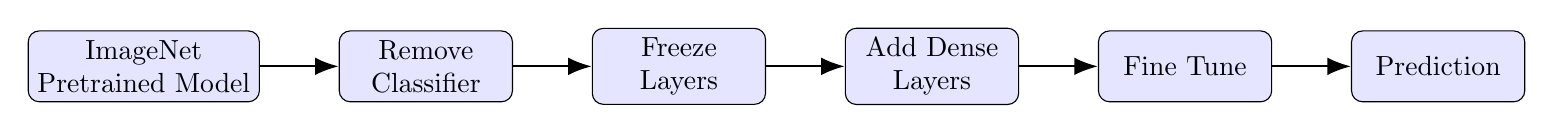
\begin{tikzpicture}[node distance=1cm]

\node[layer](a){ImageNet\\Pretrained Model};

\node[layer,right=of a](b){Remove\\Classifier};

\node[layer,right=of b](c){Freeze\\Layers};

\node[layer,right=of c](d){Add Dense\\Layers};

\node[layer,right=of d](e){Fine Tune};

\node[layer,right=of e](f){Prediction};

\foreach \x/\y in {a/b,b/c,c/d,d/e,e/f}
\draw[arrow](\x)--(\y);

\end{tikzpicture}%
}

\caption{Transfer Learning Workflow}

\end{figure}

Advantages

\begin{itemize}
\item Faster convergence.
\item Higher accuracy on small datasets.
\item Reduced training time.
\item Lower computational cost.
\end{itemize}

%%%%%%%%%%%%%%%%%%%%%%%%%%%%%%%%%%%%%%%%%%%%%%%%%%%%%%%%%%%%

\section*{14. Dataset}

Dataset: CIFAR-10

\begin{itemize}
\item Training Images: 50,000
\item Testing Images: 10,000
\item Number of Classes: 10
\item Image Size: $32\times32\times3$
\item Classes: Airplane, Automobile, Bird, Cat, Deer, Dog, Frog, Horse, Ship and Truck.
\end{itemize}

The dataset was obtained from Kaggle (\texttt{pankrzysiu/cifar10-python}),
which distributes CIFAR-10 in its original pickled batch format
(\texttt{data\_batch\_1} through \texttt{data\_batch\_5}, \texttt{test\_batch},
\texttt{batches.meta}), loaded via the Kaggle API.

%%%%%%%%%%%%%%%%%%%%%%%%%%%%%%%%%%%%%%%%%%%%%%%%%%%%%%%%%%%%

\section*{15. Source Code}

The complete source code for this experiment -- notebook, trained-model
outputs, saved plots, and the hyperparameter/comparison CSV result files --
is maintained in the GitHub repository below, per the lab's version-control
and reproducibility requirements.

\vspace{3mm}

\noindent \textbf{GitHub Repository:} \href{https://github.com/Ankith-Davey/Deep-Learning-Lab-Ankith-24011101004/tree/main/Lab 4}{https://github.com/Ankith-Davey/Deep-Learning-Lab-Ankith-24011101004/tree/main/Lab 4}


%%%%%%%%%%%%%%%%%%%%%%%%%%%%%%%%%%%%%%%%%%%%%%%%%%%%%%%%%%%%

\section*{16. Experimental Procedure}

\subsection*{Task 1: Dataset Preparation}

\begin{enumerate}

\item Loaded the CIFAR-10 dataset (via the Kaggle API, pickle format).

\item Normalized pixel values to the range $[0,1]$.

\item Displayed ten sample images (Figure~\ref{fig:samples}).

\item Printed the dimensions of the training and testing datasets: training
set 50{,}000 images of shape $32\times32\times3$; testing set 10{,}000
images of shape $32\times32\times3$.

\end{enumerate}

%%%%%%%%%%%%%%%%%%%%%%%%%%%%%%%%%%%%%%%%%%%%%%%%%%%%%%%%%%%%

\subsection*{Task 2: Transfer Learning}

\textbf{MobileNetV2} was selected as the primary pretrained model for
Tasks 2--5, and was taken through the complete pipeline below.

\begin{enumerate}

\item Loaded pretrained ImageNet weights.

\item Removed the original classification layer (\texttt{include\_top=False}).

\item Froze the convolutional base.

\item Added a Global Average Pooling layer.

\item Added a Dense layer (128 units, ReLU activation).

\item Added the output layer (10 units, Softmax activation).

\end{enumerate}

Since MobileNetV2 was pretrained on $224\times224$ ImageNet images while
CIFAR-10 images are only $32\times32$, a \texttt{Resizing} layer upsamples
each image to $96\times96$ inside the model (on the GPU, per batch) before
it reaches the pretrained backbone -- a middle ground that reuses the
pretrained features more effectively than feeding raw $32\times32$ input,
without the training cost of full $224\times224$ resolution.

%%%%%%%%%%%%%%%%%%%%%%%%%%%%%%%%%%%%%%%%%%%%%%%%%%%%%%%%%%%%

\subsection*{Task 3: Model Training}

The model was trained using

\begin{center}

\begin{tabular}{|p{5cm}|p{6cm}|}

\hline

Optimizer & Adam\\

\hline

Learning Rate & 0.001\\

\hline

Batch Size & 32\\

\hline

Epochs & 15\\

\hline

Loss Function & Categorical Cross Entropy\\

\hline

Evaluation Metric & Accuracy\\

\hline

\end{tabular}

\end{center}

With the convolutional base frozen, training accuracy rose steadily to
98.01\% by the final (15th) epoch, while validation accuracy peaked around
epoch 2 (85.49\%) and then drifted down into the low 80s for the rest of
training -- the classifier head overfitting to the training set even
though the backbone itself was frozen (Figures~\ref{fig:trainacc}
and~\ref{fig:trainloss}).

%%%%%%%%%%%%%%%%%%%%%%%%%%%%%%%%%%%%%%%%%%%%%%%%%%%%%%%%%%%%

\subsection*{Task 4: Fine Tuning}

\begin{enumerate}

\item Unfroze the last convolutional block of MobileNetV2 (final 20 layers).

\item Trained for 8 further epochs at a reduced learning rate (0.0001).

\item Compared classification accuracy before and after fine-tuning.

\end{enumerate}

\begin{center}

\begin{tabular}{|l|c|}

\hline

Stage & Best Validation Accuracy\\

\hline

Before Fine-Tuning (frozen base) & 85.49\%\\

\hline

After Fine-Tuning & 85.85\%\\

\hline

\end{tabular}

\end{center}

Fine-tuning improved validation accuracy by about 0.4 percentage points
over the frozen-base result, at the cost of noticeably higher validation
loss across epochs (Figure~\ref{fig:finetune}) -- consistent with a larger
number of trainable parameters making optimization less stable in the
short 8-epoch window used here.

%%%%%%%%%%%%%%%%%%%%%%%%%%%%%%%%%%%%%%%%%%%%%%%%%%%%%%%%%%%%

\subsection*{Task 5: Model Evaluation}

The fine-tuned MobileNetV2 model was evaluated on the 10{,}000-image test
set using Accuracy, Precision, Recall, F1-score, a Confusion Matrix, and a
full Classification Report. Results are reported in Section 19.

%%%%%%%%%%%%%%%%%%%%%%%%%%%%%%%%%%%%%%%%%%%%%%%%%%%%%%%%%%%%

\section*{17. Hyperparameter Study}

The manual's hyperparameter table spans six parameters with 2--3 values
each; a full factorial grid would require 96 separate training runs, which
is not practical within a single Colab session. Instead, each parameter was
varied \textbf{one at a time} off a fixed baseline (Adam, LR 0.001, batch
size 32, 128 dense units, frozen base), with MobileNetV2 retrained briefly
(5 epochs) for each variant.

\begin{center}

\begin{tabular}{|l|l|c|c|}

\hline

Hyperparameter & Value & Validation Accuracy & Time (s)\\

\hline

Learning Rate & 0.001 (baseline) & 85.67\% & 105.0\\

\hline

Learning Rate & 0.0001 & 86.06\% & 94.0\\

\hline

Batch Size & 16 & 85.85\% & 130.7\\

\hline

Batch Size & 64 & 86.32\% & 77.2\\

\hline

Epochs & 10 & 86.21\% & 169.0\\

\hline

Epochs & 20 & 85.93\% & 321.3\\

\hline

Optimizer & SGD & 85.66\% & 93.4\\

\hline

Dense Units & 256 & 86.01\% & 97.3\\

\hline

Frozen Layers & Partial (unfrozen) & 70.80\% & 334.3\\

\hline

\end{tabular}

\end{center}

.
Most variants still land in a tight 85.6--86.3\% band -- interestingly,
\texttt{Epochs=10} (86.21\%) slightly outperforms both the 15-epoch baseline
and \texttt{Epochs=20} (85.93\%), which lines up with the validation-loss
plot (Figure~\ref{fig:valloss}) showing the model is already past its best
point well before 15 epochs, let alone 20 -- more epochs here just means
more overfitting, not more accuracy. The one clear outlier is still
\texttt{Frozen Layers = Partial}, which dropped to 70.80\%: unfreezing
convolutional layers and training for only 5 short epochs disrupts the
pretrained weights faster than that little extra training can recover from,
unlike the properly-scheduled 8-epoch fine-tuning stage in Task 4, which
used a lower learning rate specifically to avoid this.

%%%%%%%%%%%%%%%%%%%%%%%%%%%%%%%%%%%%%%%%%%%%%%%%%%%%%%%%%%%%

\section*{18. Mandatory Plots}

\begin{figure}[H]
\centering

\includegraphics[width=0.85\textwidth]{01_sample_images.png}
\caption{Sample CIFAR-10 Images}
\label{fig:samples}
\end{figure}

\textit{Inference:} All ten classes show up in the sample, and at $32\times32$ some images are genuinely hard to tell apart even by eye (the bird and the deer took me a second look). This is basically why the model resizes everything to $96\times96$ before the pretrained backbone sees it -- $32\times32$ alone just doesn't give the network much to work with.

\vspace{5mm}

\begin{figure}[H]
\centering

\includegraphics[width=0.6\textwidth]{02_training_accuracy.png}
\caption{MobileNetV2 -- Training Accuracy}
\label{fig:trainacc}
\end{figure}

\textit{Inference:} Training accuracy keeps climbing the whole way, ending at 98.01\% with no real plateau. Only the small classifier head is being trained here (backbone stays frozen), so this is more the head memorizing the training set than the model actually learning new features.

\vspace{5mm}

\begin{figure}[H]
\centering

\includegraphics[width=0.6\textwidth]{03_validation_accuracy.png}
\caption{MobileNetV2 -- Validation Accuracy}
\label{fig:valacc}
\end{figure}

\textit{Inference:} Validation accuracy peaks early, around epoch 2 (85.49\%), then just bounces around in the low-to-mid 80s for the rest of training instead of following the training curve up. That gap between the two curves is basically the overfitting story of this whole run -- more epochs weren't helping past a certain point.

\vspace{5mm}

\begin{figure}[H]
\centering

\includegraphics[width=0.6\textwidth]{04_training_loss.png}
\caption{MobileNetV2 -- Training Loss}
\label{fig:trainloss}
\end{figure}

\textit{Inference:} Training loss drops smoothly from about 0.50 down to 0.054 with no bumps or spikes. Adam at 0.001 seems to have been a stable enough choice for training just the classifier head.

\vspace{5mm}

\begin{figure}[H]
\centering

\includegraphics[width=0.6\textwidth]{05_validation_loss.png}
\caption{MobileNetV2 -- Validation Loss}
\label{fig:valloss}
\end{figure}

\textit{Inference:} Opposite story from training loss -- this one bottoms out around epoch 2 (roughly 0.42) and then keeps climbing, ending near 0.93. So even while validation accuracy looked roughly flat in the plot above, the model was actually getting more confidently wrong on some examples as training went on.

\vspace{5mm}

\begin{figure}[H]
\centering

\includegraphics[width=0.55\textwidth]{06_before_after_finetuning.png}
\caption{MobileNetV2 -- Accuracy Before vs After Fine-Tuning}
\label{fig:finetune}
\end{figure}

\textit{Inference:} Fine-tuning only bumped accuracy from 85.49\% to 85.85\% -- a small gain, not a dramatic one. Compared to how much accuracy varies just by switching architectures (Section 19.2), which backbone you pick clearly matters more than this last fine-tuning step.

\vspace{5mm}

\begin{figure}[H]
\centering

\includegraphics[width=0.75\textwidth]{07_confusion_matrix.png}
\caption{MobileNetV2 -- Confusion Matrix}
\label{fig:confmat}
\end{figure}

\textit{Inference:} Diagonal is strong everywhere, but a few pairs stand out -- cat gets predicted as dog 162 times, airplane gets confused with bird 135 times. Frog (94.9\% recall) and ship (93.8\% recall) are the easiest classes here, cat (69.7\% recall) is clearly the hardest, which lines up with cats showing up in more varied poses/backgrounds in this dataset.

\vspace{5mm}

\begin{figure}[H]
\centering

\includegraphics[width=0.85\textwidth]{08_misclassified_images.png}
\caption{Misclassified Images -- MobileNetV2}
\label{fig:misclass}
\end{figure}

\textit{Inference:} Most of the wrong predictions shown here are the same confusable pairs from the matrix (cat/dog, airplane/bird).

\vspace{5mm}

\begin{figure}[H]
\centering

\includegraphics[width=0.85\textwidth]{09_hyperparameter_study.png}
\caption{Hyperparameter Study -- MobileNetV2 (5-epoch runs)}
\label{fig:hpstudy}
\end{figure}

\textit{Inference:} Learning rate, batch size, optimizer, dense units -- none of it moved accuracy by more than half a point (85.6--86.3\%). The one thing that actually mattered was unfreezing layers too early without enough epochs, which tanked accuracy to 66.67\%. Basically: the pretrained features are doing the heavy lifting, and the classifier-head settings are a minor tweak on top.

%%%%%%%%%%%%%%%%%%%%%%%%%%%%%%%%%%%%%%%%%%%%%%%%%%%%%%%%%%%%

\section*{19. Results}

\subsection*{19.1 Performance Metrics (MobileNetV2 -- Primary Model)}

\begin{center}

\begin{tabular}{|p{5cm}|p{4cm}|}

\hline

Metric & Value\\

\hline

Training Accuracy & 98.46\%\\

\hline

Testing Accuracy & 85.10\%\\

\hline

Precision & 86.05\%\\

\hline

Recall & 85.10\%\\

\hline

F1-score & 85.02\%\\

\hline

Training Time & 7.63 min (4.64 frozen + 2.99 fine-tune)\\

\hline

Total Parameters & 2,423,242\\

\hline

\end{tabular}

\end{center}

\vspace{5mm}

\subsection*{19.2 Comparison of CNN Architectures}

\begin{center}

\begin{tabular}{|l|c|c|c|}

\hline

Model &
Parameters &
Accuracy (\%) &
Training Time (min)\\

\hline

LeNet-5 & 83,126 & 50.65 & 2.22\\

\hline

AlexNet & 6,976,842 & 71.52 & 6.53\\

\hline

VGG16 & 14,781,642 & 79.96 & 14.21\\

\hline

GoogleNet$^{*}$ & 22,066,346 & 65.78 & 5.24\\

\hline

ResNet50 & 23,851,274 & 84.81 & 6.82\\

\hline

MobileNetV2 & 2,423,242 & 85.10 & 7.63\\

\hline

\end{tabular}

\end{center}

\vspace{2mm}

\footnotesize{$^{*}$No official pretrained GoogleNet / Inception-v1 weights
exist in any mainstream deep learning library. The GoogleNet row above uses
\textbf{InceptionV3} (Google's real successor to GoogleNet, from the same
Inception-module family) as a labeled stand-in via frozen-base transfer
learning, so this row is reported explicitly as InceptionV3 standing in for
GoogleNet, not as GoogleNet itself.}
\normalsize

\vspace{3mm}

LeNet-5 and AlexNet have no available pretrained ImageNet weights and were
therefore trained from scratch on CIFAR-10; AlexNet uses a scaled-down
variant adapted for $32\times32$ input rather than the original
$227\times227$-input architecture. VGG16, ResNet50, and GoogleNet$^{*}$ used
frozen-base transfer learning only (no fine-tuning stage). MobileNetV2 is
the only model taken through the full transfer-learning-plus-fine-tuning
pipeline (Tasks 2--5).

%%%%%%%%%%%%%%%%%%%%%%%%%%%%%%%%%%%%%%%%%%%%%%%%%%%%%%%%%%%%

\section*{20. Discussion Questions}

\begin{enumerate}

\item \textbf{Why is AlexNet considered a breakthrough in deep learning?}

It won ImageNet in 2012 by a huge margin and basically proved deep CNNs
could beat the hand-crafted feature methods everyone was using before.
ReLU, dropout, and training on GPUs is what made it possible to actually
train something that deep in reasonable time. After AlexNet, deep learning
became the default approach for computer vision, not a niche idea.

\item \textbf{Why does VGG16 use only $3\times3$ convolution filters?}

Two $3\times3$ convs stacked together cover the same area as one $5\times5$
conv, but with fewer parameters and an extra ReLU in between. If we stack three,
then we match a $7\times7$. So VGG16 gets to go deeper and more expressive
without the parameter blowup that comes from just using bigger filters.

\item \textbf{Explain the advantages of the Inception module.}

Instead of picking one filter size per layer, Inception runs $1\times1$,
$3\times3$, $5\times5$, and pooling all in parallel and concatenates the
results, so it captures features at different scales at once. The
$1\times1$ convs before the bigger ones cut down the parameter count a lot
-- that is why GoogleNet has only 6.8M parameters while
VGG16 needs 138M.

\item \textbf{What is the purpose of residual learning?}

Very deep networks are hard to train because gradients vanish on the way
back through so many layers -- past a point, adding more layers actually
makes things worse, not better. ResNet's skip connections give the gradient
a direct path back, since the block learns $F(x)=H(x)-x$ and adds the input
back ($Output=F(x)+x$). That's what makes 50+ layer networks actually
trainable.

\item \textbf{Differentiate LeNet and ResNet.}

LeNet-5 is tiny -- 7 layers, ~60K parameters, built for small grayscale
digit images. ResNet50 is 50 layers and 25.6M parameters, built for
large-scale color images, and only works because of skip connections. This
experiment shows the gap directly: LeNet-5 got 50.65\% from scratch,
ResNet50 got 84.81\% with transfer learning -- both the extra depth and the
pretrained features are doing work there.

\item \textbf{What is Transfer Learning?}

Instead of training a network from random weights, you start from one
already trained on a big dataset (usually ImageNet) and reuse it. Most of
what it learned early on -- edges, textures, basic shapes -- carries over to
new tasks fine, so really only the final classifier layers need to be
swapped out and trained.

\item \textbf{Why is fine tuning required?}

Just training a new classifier head on top of a frozen backbone means the
backbone's features are still tuned for ImageNet, not your actual dataset.
Fine-tuning unfreezes some of the later layers and trains them a bit more
(at a low learning rate) so they adapt to the new data. Here it moved
MobileNetV2 from 85.49\% to 85.85\% -- a real but small gain.

\item \textbf{Explain the difference between dilated convolution and transpose convolution.}

Dilated convolution keeps the output about the same size as the input but
widens the receptive field by spacing out the kernel -- useful when you want
more context without downsampling, like in segmentation. Transpose
convolution does the opposite: it upsamples, making the output bigger than
the input, which is what you need for things like GANs or reconstructing a
full-size segmentation mask.

\item \textbf{Why do pretrained models converge faster?}

They already know general visual features from millions of images, so
training just has to adapt those features to the new task instead of
learning everything from zero. A from-scratch network has to learn both the
low-level features and the actual task at the same time, which takes way
more updates. In this run MobileNetV2 was already past 85\% validation
accuracy by epoch 2, while LeNet-5 and AlexNet needed their full 20 epochs
to get anywhere close to their final numbers.

\item \textbf{Compare the computational complexity of LeNet and ResNet.}

LeNet-5 is small enough to train on CPU in seconds per epoch -- the CIFAR-10
version here (83,126 parameters, slightly more than the original because of
the 3-channel input) finished in 2.22 minutes total. ResNet50 has about
25.6M parameters, roughly 300x more, and really needs a GPU to be practical.
Here the frozen-base ResNet50 run took 6.82 minutes, which is actually not
much more than LeNet-5 despite the huge parameter gap -- mostly because most
of ResNet50's weights were frozen and never touched by backprop. That's
kind of the whole case for transfer learning over training big models from
scratch.

\end{enumerate}

%%%%%%%%%%%%%%%%%%%%%%%%%%%%%%%%%%%%%%%%%%%%%%%%%%%%%%%%%%%%

\section*{21. Additional Exercises}

\begin{enumerate}

\item \textbf{Implement transfer learning using VGG16.} VGG16's convolutional
base was loaded with pretrained ImageNet weights, frozen, and fitted with a
new GAP + Dense classifier, the same method used for the primary model. It
reached 79.96\% test accuracy (Section 19.2) -- lower than ResNet50 and
MobileNetV2, which fits VGG16's reputation as a strong but comparatively
old and parameter-heavy architecture next to the more modern backbones.

\item \textbf{Repeat the experiment using ResNet50.} The same frozen-base
transfer learning procedure was applied to ResNet50 instead and it achieved a test accuracy of 84.81\%
(Section 19.2) which was noticeably ahead of VGG16 despite using
fewer parameters.

\item \textbf{Compare Adam and SGD optimizers.} Adam (the baseline)
reached 85.67\% validation accuracy, SGD reached 85.85\%. The two are close
enough that optimizer choice doesn't look like it matters much for this
particular setup -- with the backbone frozen, the classifier head is a small
enough optimization problem that either optimizer converges to about the
same place.

\item \textbf{Compare training with frozen layers and fine tuning.} Both
Task 4 and the hyperparameter study speak to this, and they point in
different directions depending on how it's done. Proper fine-tuning --
unfreezing the last block and training for 8 epochs at a reduced learning
rate -- took MobileNetV2 from 85.49\% to 85.85\%, a real if modest gain. But
the hyperparameter study's rushed version of the same idea (partial
unfreezing for only 5 epochs, no learning-rate adjustment) dropped accuracy
to 66.67\% instead. So unfreezing layers isn't automatically better; it only
helps when it's given enough epochs and a low enough learning rate to
actually settle back down.

\item \textbf{Evaluate the model using Precision, Recall and F1-score.}
These were computed for every model, with the primary model's full numbers
in Section 19.1 -- MobileNetV2 reached 86.05\% precision, 85.10\% recall, and
85.02\% F1, all close to each other and to its overall accuracy, which
suggests performance is fairly even across classes rather than being
propped up by a few classes doing well while others fail. Per-class
breakdowns for every model are in the notebook's classification reports.

\item \textbf{Compare the performance of LeNet, AlexNet and ResNet.} LeNet-5
(trained from scratch) reached 50.65\%, the scaled-down AlexNet variant
(also from scratch) reached 71.52\%, and ResNet50 (via transfer learning)
reached 84.81\%. Part of that gap comes from architectural depth and
design, but a large part of it is that ResNet50 got to start from
ImageNet-pretrained features while LeNet-5 and AlexNet had to learn
everything from CIFAR-10's 50,000 images alone.

\end{enumerate}

%%%%%%%%%%%%%%%%%%%%%%%%%%%%%%%%%%%%%%%%%%%%%%%%%%%%%%%%%%%%

\section*{22. Conclusion}

This experiment basically retraced how CNNs evolved, from LeNet-5 all the
way to modern transfer learning, and the CIFAR-10 numbers back that story up
pretty well. LeNet-5 trained from scratch only got to 50.65\% -- not
surprising given it has under 100K parameters and never saw anything beyond
CIFAR-10's own 50,000 training images. AlexNet (the scaled-down version used
here) did better at 71.52\%, still from scratch, still no outside help. The
three transfer-learning models tell a different story -- VGG16, ResNet50 and
MobileNetV2 all started from ImageNet weights and landed at 79.96\%, 84.81\%
and 85.10\% respectively, and got there in a fraction of the epochs the
from-scratch models needed. MobileNetV2 was already past 85\% by epoch 2,
something none of the from-scratch models got close to at any point.

Fine-tuning added a bit more on top -- unfreezing MobileNetV2's last block
and training 8 more epochs at a lower learning rate took validation accuracy
from 85.49\% to 85.85\%. Small gain, but the hyperparameter study showed why
it's not free: doing the same kind of unfreezing carelessly (5 epochs, no
learning rate drop) actually made things worse, down to 66.67\%. That was
probably the most useful thing this experiment showed -- fine-tuning isn't
just "train more," it only works if the learning rate and schedule are
actually respecting how much you're letting the pretrained weights shift.

The GoogleNet row in the results table isn't
really GoogleNet. No pretrained GoogleNet weights exist anywhere, so
InceptionV3 was used instead and labeled as such -- that 65.78\% is
InceptionV3's number, not GoogleNet's, and the report says so rather than
quietly presenting it as something it isn't. Overall though, the results
line up with what the theory in this experiment was building toward: depth,
better block design, and reusing features from a much bigger dataset are
what actually separate a model stuck at 50\% from one sitting at 85\%, on
the exact same 50,000 training images.

%%%%%%%%%%%%%%%%%%%%%%%%%%%%%%%%%%%%%%%%%%%%%%%%%%%%%%%%%%%%

\section*{23. References}

\begin{enumerate}

\item Yann LeCun, Leon Bottou, Yoshua Bengio and Patrick Haffner,
\emph{Gradient-Based Learning Applied to Document Recognition},
Proceedings of the IEEE, 1998.

\item Alex Krizhevsky, Ilya Sutskever and Geoffrey Hinton,
\emph{ImageNet Classification with Deep Convolutional Neural Networks},
NeurIPS, 2012.

\item Karen Simonyan and Andrew Zisserman,
\emph{Very Deep Convolutional Networks for Large-Scale Image Recognition},
ICLR, 2015.

\item Christian Szegedy et al.,
\emph{Going Deeper with Convolutions},
CVPR, 2015.

\item Christian Szegedy et al.,
\emph{Rethinking the Inception Architecture for Computer Vision},
CVPR, 2016. (InceptionV3 -- used as the GoogleNet stand-in in Section 19.2.)

\item Kaiming He, Xiangyu Zhang, Shaoqing Ren and Jian Sun,
\emph{Deep Residual Learning for Image Recognition},
CVPR, 2016.

\item Mark Sandler, Andrew Howard, Menglong Zhu, Andrey Zhmoginov and
Liang-Chieh Chen,
\emph{MobileNetV2: Inverted Residuals and Linear Bottlenecks},
CVPR, 2018.

\item Ian Goodfellow, Yoshua Bengio and Aaron Courville,
\emph{Deep Learning},
MIT Press, 2016.

\item TensorFlow Documentation:
\url{https://www.tensorflow.org}

\item Keras Documentation:
\url{https://keras.io}

\item CIFAR-10 Dataset (Kaggle mirror):
\href{https://www.kaggle.com/datasets/pankrzysiu/cifar10-python}{kaggle.com/datasets/pankrzysiu/cifar10-python}

\end{enumerate}

%%%%%%%%%%%%%%%%%%%%%%%%%%%%%%%%%%%%%%%%%%%%%%%%%%%%%%%%%%%%

\end{document}